\chapter{Simulation 3D sous Ansys Electronics HFSS}

\section{Objectif}

L'objectif de ce TP est de se familiariser avec le logiciel de simulation Ansys Electronics, et plus particulièrement le module de simulation Electromagnétique 3D HFSS\@. Nous allons apprendre à créer un modèle d'antenne, à définir les conditions aux limites appropriées, à effectuer des simulations électromagnétiques et à interpréter les résultats obtenus.

\section{Préparation}

L'objectif de cette préparation est de vous familiariser avec le logiciel. 

Voici le lien vers un tutoriel de Ansys HFSS pour la simulation d'un guide d'onde:

\href{https://www.youtube.com/playlist?list=PLtt6-ZgUFmMIALOB6FTW9n3HbMwOoGJQ4}{www.youtube.com/playlist?list=PLtt6-ZgUFmMIALOB6FTW9n3HbMwOoGJQ4}

\vspace{0.5cm}
Une version étudiante du logiciel peut être téléchargée ici:

\href{https://ansys.synopsys.com/academic/students/ansys-student}{https://ansys.synopsys.com/academic/students/ansys-student}
\section{Modélisation d'une antenne quart d'onde avec plan de masse infini}

L'objectif de cette partie est de modéliser une antenne monopole quart d'onde avec un plan de masse de infini.

Vous pouvez vous inspirer du tutoriel suivant pour créer votre antenne. Attention cependant, nous souhaitons créer une antenne monopole et non dipôle!

\href{https://www.youtube.com/watch?v=dUC720AJvK0}{https://www.youtube.com/watch?v=dUC720AJvK0}

\subsection{Modélisation de l'antenne}

\begin{itemize}
    \item Créer un nouveau projet et insérer un nouveau ``HFSS Design''.

    \newpage
    \item Créer la liste des paramètres suivants dans le design HFSS en faisant un click droit sur design HFSS $\rightarrow$ ``Design Properties''. Faire ``Add Properties'' pour ajouter une nouvelle variable. On prendra soin de préciser le type et l'unité de chaque variable.

\begin{center}
\begin{tabular}{|l|l|}  %chktex 44
\hline %chktex 44
\textbf{Name} & \textbf{Expression} \\
\hline %chktex 44
$f0$ & 2 GHz \\
%\hline %chktex 44
%$c$ & 3e8[m/s] \\
\hline %chktex 44
$lambda$ & $c0/f0$ \\
\hline %chktex 44
$h\_ant$ & 35 mm \\
\hline %chktex 44
$r\_ant$ & 0.65 mm \\
%\hline %chktex 44
%$r\_GND$ & 0.18 m \\
\hline %chktex 44
$r\_coax$ & 2.2 mm \\
\hline %chktex 44
%$h\_GND$ & 0.5 mm \\
%\hline %chktex 44
%$r\_calcul$ & 2*lambda\\
%\hline %chktex 44
$h\_coax$ & 0.1 mm \\
\hline %chktex 44
\end{tabular}
\end{center}

% \begin{itemize}
%     \item Fréquence de travail: $f_0$: 2[GHz]
%     \item Vitesse de la lumière: $c$: 3e8[m/s]
%     \item Longueur d'onde: $\lambda_0$: = $c/f_0$
%     \item Longueur de l'antenne: $h_{ant}$: 35[mm]
%     \item Rayon de l'antenne: $r_{ant}$: 0.65[mm]
%     \item Plan de masse circulaire de rayon $r_{GND}$: 0.18[m] (\textit{on fera varier ce paramètre par la suite})
%     \item Rayon du coaxial d'alimentation: $r_{coax}$: 2.2[mm]
% \end{itemize}

    \item Créer la géométrie de l'antenne quart d'onde et du coaxial d'alimentation en utilisant les paramètres créés précédament. Leur assigner les matériaux correspondant: ``pec'' pour le monopôle et ``teflon\_based'' pour le coaxial.

    \begin{figure}[H]
        \centering
        
\includegraphics[width=0.8\textwidth]{TP_Simulation_HFSS/fig/monopole_coax.png}
    \end{figure}

    %\item Créer le plan de masse.

    \item Définir le port d'excitation: pour cela sélectionner la surface correspondant à l'entrée du coaxial $\rightarrow$ ``Assign Excitation'' $\rightarrow$ ``Port'' $\rightarrow$ ``Modal Wave Port''. Attention à coher la case ``Spécify Direction'' et à vérifier que la direction est la bonne.

    \begin{figure}[H]
        \centering
        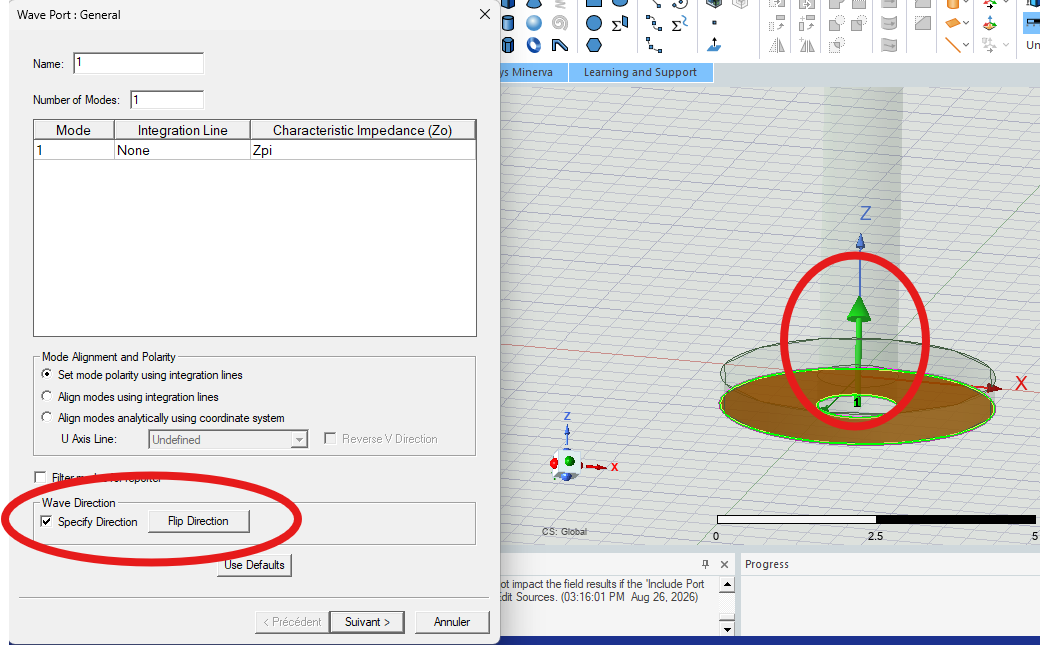
\includegraphics[width=0.8\textwidth]{TP_Simulation_HFSS/fig/Port.png}
    \end{figure}

    \item Définir les conditions aux limites: click droit ``Create Open Region'' et indiquer une fréquence de travail de 2 GHz et une limite de type ``PML''. Afin de simuler un plan de masse infini, cocher la case ``Apply infinite ground plane at''.
    
    Remarque: \textit{``Compared to Radiation boundaries, which create absorbing boundary conditions (ABC), PMLs in general make it more difficult for the iterative solver to reach convergence compared to the same model with using ABCs. PMLs also require significantly more RAM\@. The advantages for PMLs are that they absorb a much wider range of waves in terms of frequency and direction. As a result, you can put PMLs much closer to the discontinuities. This gives a smaller model. ABCs efficiently absorb normal incident waves. You have to put ABCs far away enough from the discontinuities''}
     
    \begin{figure}[H]
        \centering
        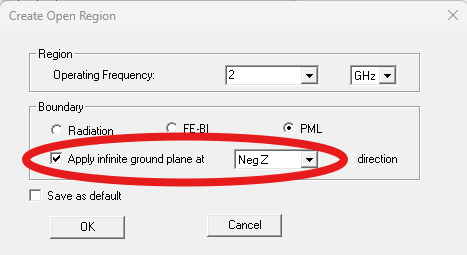
\includegraphics[width=0.72\textwidth]{TP_Simulation_HFSS/fig/Boundaries_infinite.png}
    \end{figure}

    \item Définir la simulation: click droit sur ``Analysis'' $\rightarrow$ ``Add Solution Setup'' $\rightarrow$ ``Advanced\ldots'' 
    
    \begin{figure}[H]
        \centering
        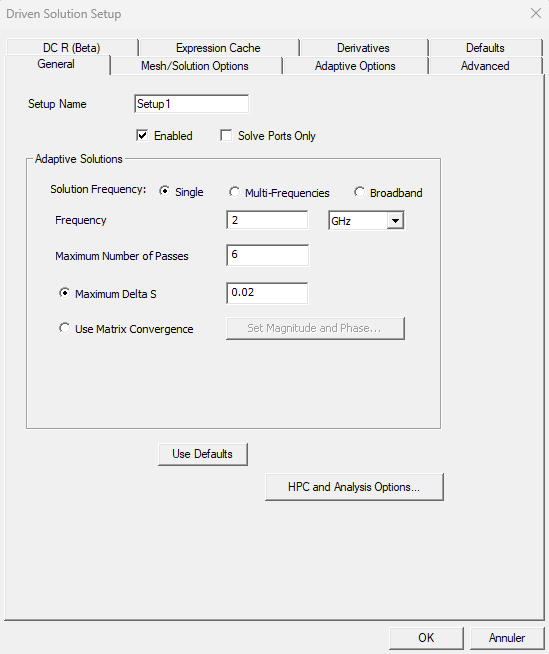
\includegraphics[width=0.75\textwidth]{TP_Simulation_HFSS/fig/Simu_param.png}
    \end{figure}

    Cette partie concerne la définition du maillage de simulation. Ce logiciel permet de réaliser une simulation 3D avec la méthode des éléments finis. Cela signifie que la structure est maillée afin de calculer de proche en proche les grandeurs physiques dans chaque maille. Si les mailles sont trop petites, il y aura énormément de calculs à faire car un grand nombre de maille sera nécessaire pour mailler la structure à simuler. Si les mailles sont trop grandes, les résultats de la simulation ne seront pas précis, voir complétement différent de la réalité.
    \begin{itemize}
        \item Onglet ``General'': paramètres généraux pour la création du maillage. On peut ainsi définir les paramètres de convergence à partir duquel on considère le maille suffisant pour notre simulation. Plus ce paramètre sera petit, plus le résultat sera précis. On choisit typiquement un Delta S de 0.01 à 0.02.
        \item Onglet ``Mesh/Solution Setup'': ce sont les options avancées pour le raffinement du maillage
    \end{itemize}

    \newpage
    Après validation des paramètres du maillage, une nouvelle fenêtre s'ouvre afin de définir les paramètres de la simulation: fréquences\ldots ATTENTION\@: pensez à cocher la case ``Save Fields'' afin d'avoir accès aux champs (Electrique, magnétique et rayonnement). Vous pouvez éventuellemnt n'enregistrer que le champ rayonné sur le champ proche ne vous intéresse pas (permet d'avoir des résultats de simulation prenant moins d'espace disque).

    \item Avant de lancer la simulation, vérifier que tout est paramétré: aller dans ``Simulation'' et cliquer sur ``Validate''. Si tout est bon, vous pouvez lancer la simulation en cliquant sur `` Analyse All''. Pendant la simulation, vous pouvez observer la vitesse de convergence. Pour cela faites un clic droit sur ``Setup1'' et sélectionnez ``Convergence\ldots''. Vous pouvez entre autre afficher la convergence sous forme de ``Plot''.

\end{itemize}

\subsection{Vérifications des résultats}

\begin{itemize}
    \item Vérifiez dans un premier temps que le mode d'excitation du coaxial est bon. Pour cela, cliquez sur ``Port Field Display'' $\rightarrow$ ``Mode 1'' et observez le champ E. Commentez.
    
    \item Vérifiez l'impédance du port d'entrée. Pour cela, cliquez sur ``Results'' $\rightarrow$ ``Create Modal Solution Data Report'' $\rightarrow$ ``Rectangular Plot'' et sélectionnez le paramètre ``Port Zo''. Au vu des dimentions du coaxial, l'impédance devrait être de 50 $\Omega$.
    
    \item Notez la fréquence de résonnance de l'antenne et son impédance d'entrée à cette fréquence. Vérifiez cette valeur avec la formule théorique de l'antenne quart d'onde. Commentez.
    
    \item Observez le diagramme de rayonnement de l'antenne (3D et plans de coupe) ainsi que les valeurs maximales de la directivité et du gain. Commentez. Quelle est la polarisation de l'antenne? Donner le ratio Co-polar / Cross-polar.
    

\end{itemize}

\section{Modélisation d'une antenne quart d'onde avec plan de masse de taille finie}

Nous allons maintenant étudier les effets de la taille du plan de masse sur les performances de l'antenne, notamment sur son impédance d'entrée, son gain et son diagramme de rayonnement.

\begin{itemize}
    \item Afin de garder la simulation précédente, copiez le design précédent dans le même projet.
    
    \item Ajouter un plan de masse avec les dimensions suivantes (ajoutés aux paramètres de la simulation):
    
    \begin{center}
    \begin{tabular}{|l|l|}  %chktex 44
    \hline %chktex 44
    \textbf{Name} & \textbf{Expression} \\
    \hline %chktex 44
    $r\_GND$ & 0.18 m \\
    $h\_GND$ & 0.5 mm \\
    \hline %chktex 44
    \end{tabular}
    \end{center}

    \item Retirez la condition aux limites de plan de masse infini (garder la condition PML). Attention, pour cela il faut supprimer le \textit{PMLGroup} dans le \textit{Model} pour le recréer.

 \end{itemize}

\subsection{Vérifications des résultats}

\begin{itemize}
    \item Vérifiez dans un premier temps que le mode d'excitation du coaxial et l'impédance du port sont toujours bons.
    
    \item Notez la fréquence de résonnance de l'antenne et son impédance à cette fréquence. Commentez.
    
    \item Observez le diagramme de rayonnement de l'antenne ainsi que les valeurs maximales de la directivité et du gain. Commentez.
    
    \item Reprendre les question précédentes pour un plan de masse de rayon 0.1 m, 0.05 m puis 0.01 m. Commentez.
\end{itemize}